We developed the application using both server-side and client-side programming. This chapter presents both sides of the programming, starting with describing the adjustments made to the design based on findings from Study II. Privacy and security considerations and implementation are described at the end of the chapter. The developed application can be found on attached CD.

\section{Design Changes}

\begin{figure}[h]
  \centering
  \begin{minipage}[b]{0.45\textwidth}
    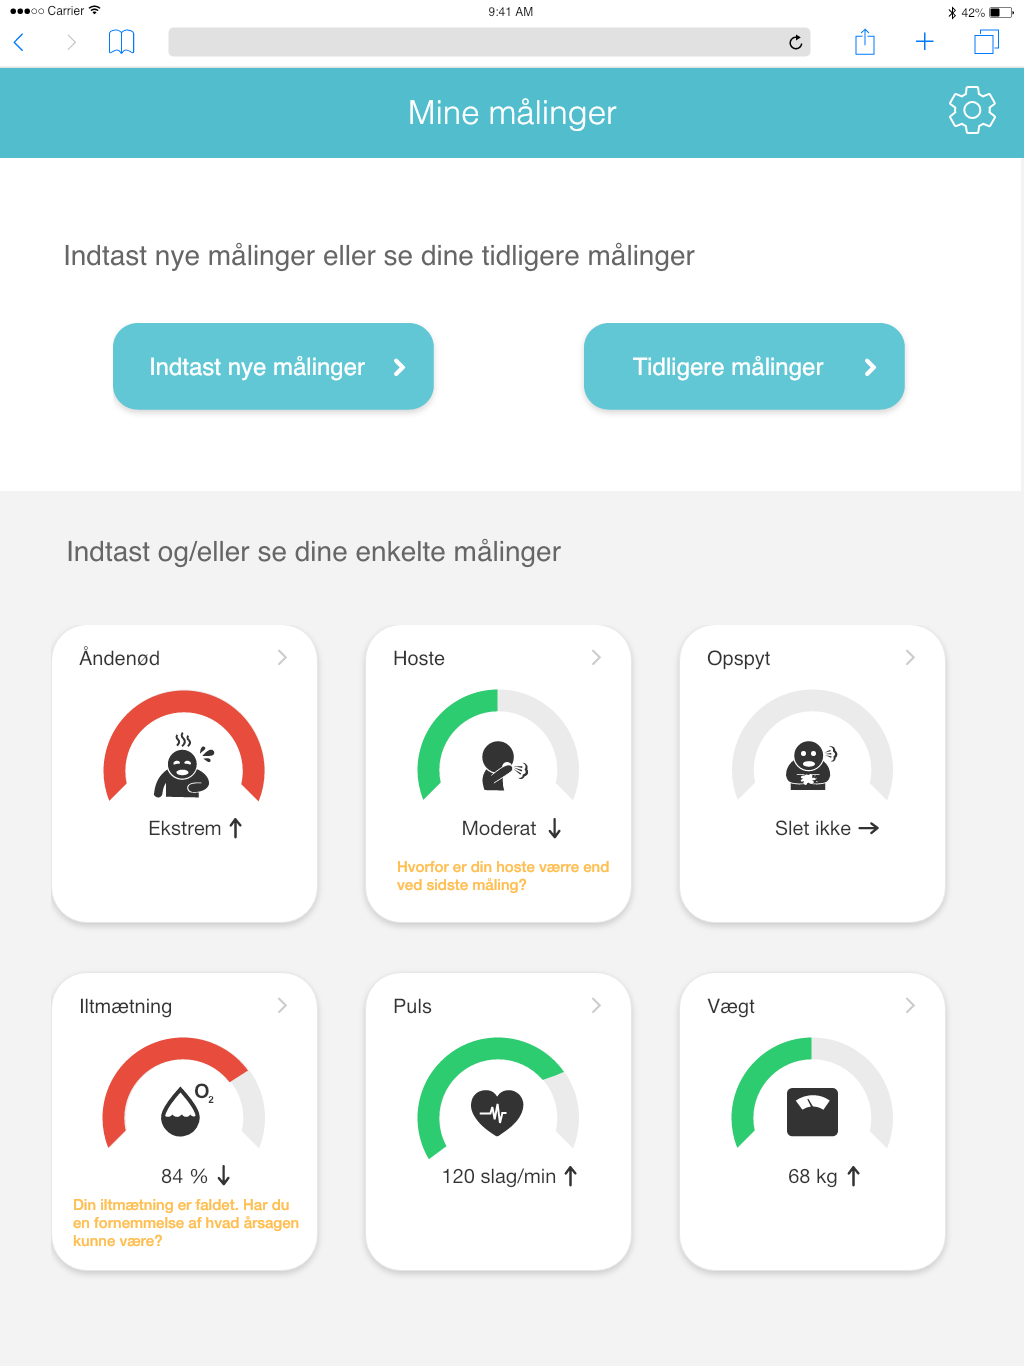
\includegraphics[width=\textwidth]{images/study2/Dashboard.png}
    \caption{Dashboard used in Study II}
    \label{fig:db1st}
  \end{minipage}
  \hfill
  \begin{minipage}[b]{0.45\textwidth}
    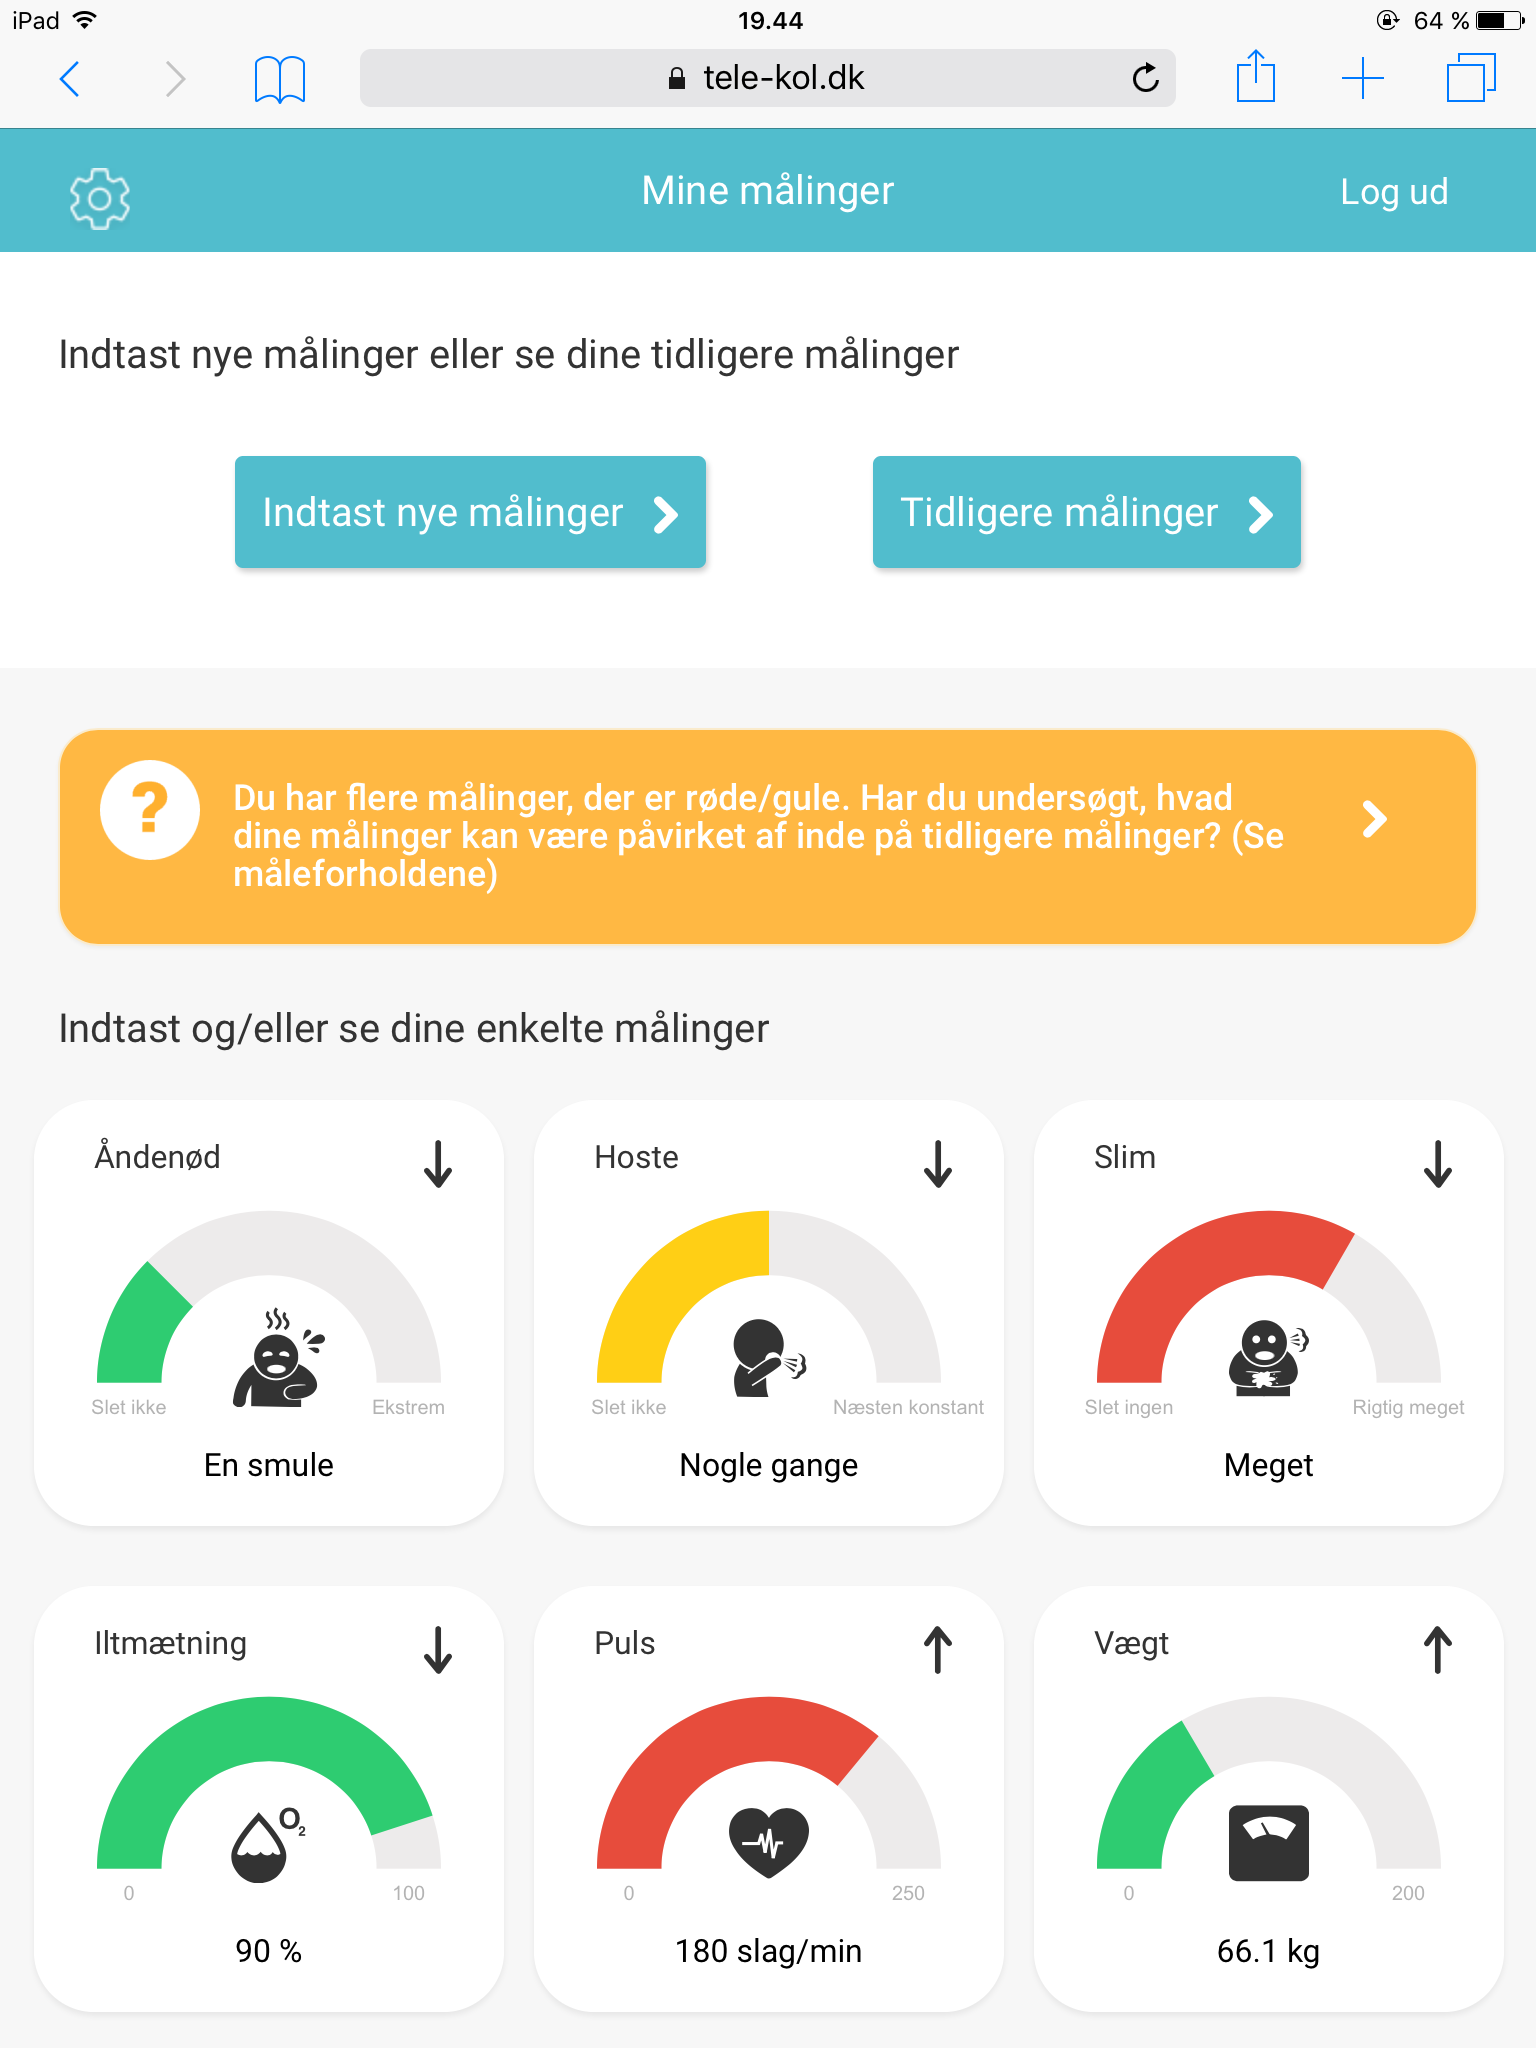
\includegraphics[width=\textwidth]{images/implementation/db.PNG}
    \caption{Redesigned dashboard}
    \label{fig:db2nd}
  \end{minipage}
\end{figure}

\subsection*{Reflective Questions}
Reflective questions were measure-specific in our first design proposal as seen on Figure \ref{fig:db1st}. We found in Study II that patients did not notice the reflective questions and thus decided to redesign the reflective questions as seen on Figure \ref{fig:db2nd}. 

Reflective questions were redesigned to target overall health status and updated depending on following conditions: 
 
\paragraph{When all color indicators were green (or only one yellow/red)}
\begin{itemize}
\item When should you be extra aware of your symptoms?
\item What is the status on your measures?
\item Is there any improvement in your latest measures? (Look at the arrows on each measure)
\item Have you explored what your measures might have been affected by in previous measures? (See measurement conditions)
\item Have you examined whether your normal range is adjusted to your needs? (Look at settings gear in the upper left corner)
\end{itemize}

\paragraph{When at least two measures were yellow/red}
\begin{itemize}
\item (You have multiple measures showing red/yellow.) Have you previously been able to improve your measures? How? 
\item (You have multiple measures showing red/yellow.) Which measures should you be aware of?
\item (You have multiple measures showing red/yellow.) How are your responses when you feel well?
\item You have multiple measures showing red/yellow. How long have your measures been like this? Is there anything you should be aware of?
\item You have multiple measures showing red/yellow. Is there any improvement in your latest measures? (Look at the arrows on each measure)
\item You have multiple measures showing red/yellow. Have you explored what your measures might have been affected by in previous measures? (See measurement conditions)
\item You have multiple measures showing red/yellow. Have you examined whether your normal range is adjusted to your needs? (Look at settings gear in the upper left corner)
\end{itemize}

\subsection*{Visualisation Choice}
We provided patients with four visualisations and from the feedback found that patients had different preferences. Based on findings from literature and patients' statements about the visualisations, we chose Visualisation 1 for long-term reflection (See Figure \ref{fig:visualization}). 
 
\subsection*{Normal Area}
Based on findings from previous research and findings from Study I showing that patients preferred their own normal area. we provided the patients with a settings option to individualize the normal area for each objective measure (See Figure \ref{fig:settings}). 

\begin{figure}[h]
  \centering
  \begin{minipage}[b]{0.45\textwidth}
    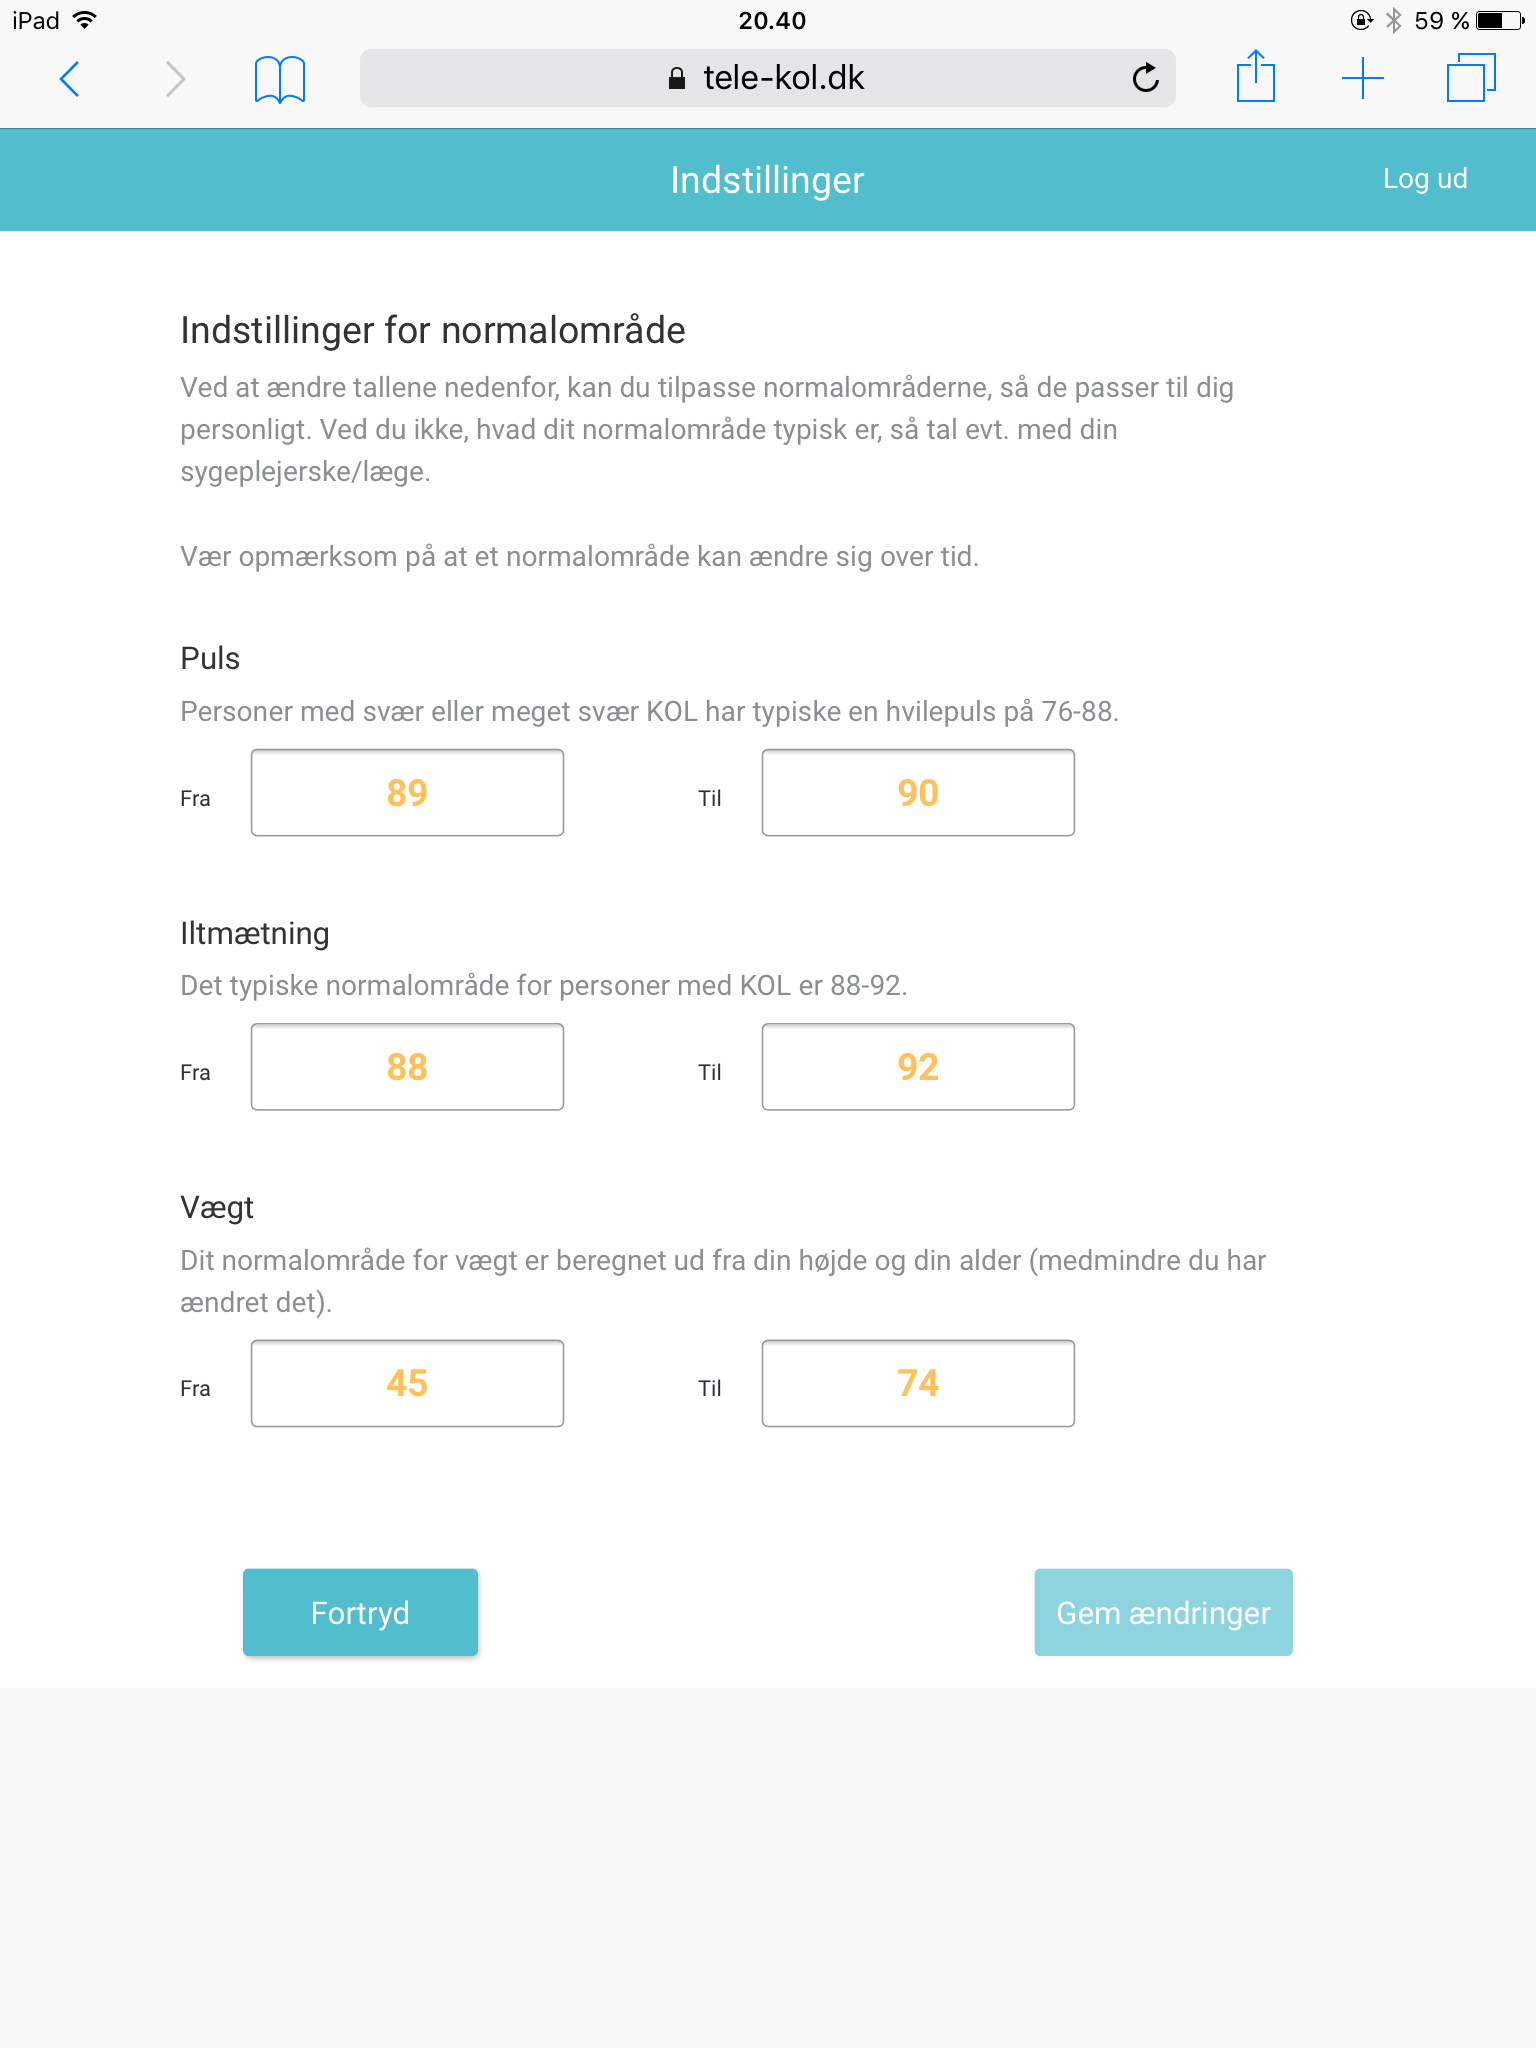
\includegraphics[width=\textwidth]{images/implementation/settingsImp.png}
    \caption{Settings}
    \label{fig:settings}
  \end{minipage}
  \hfill
  \begin{minipage}[b]{0.45\textwidth}
    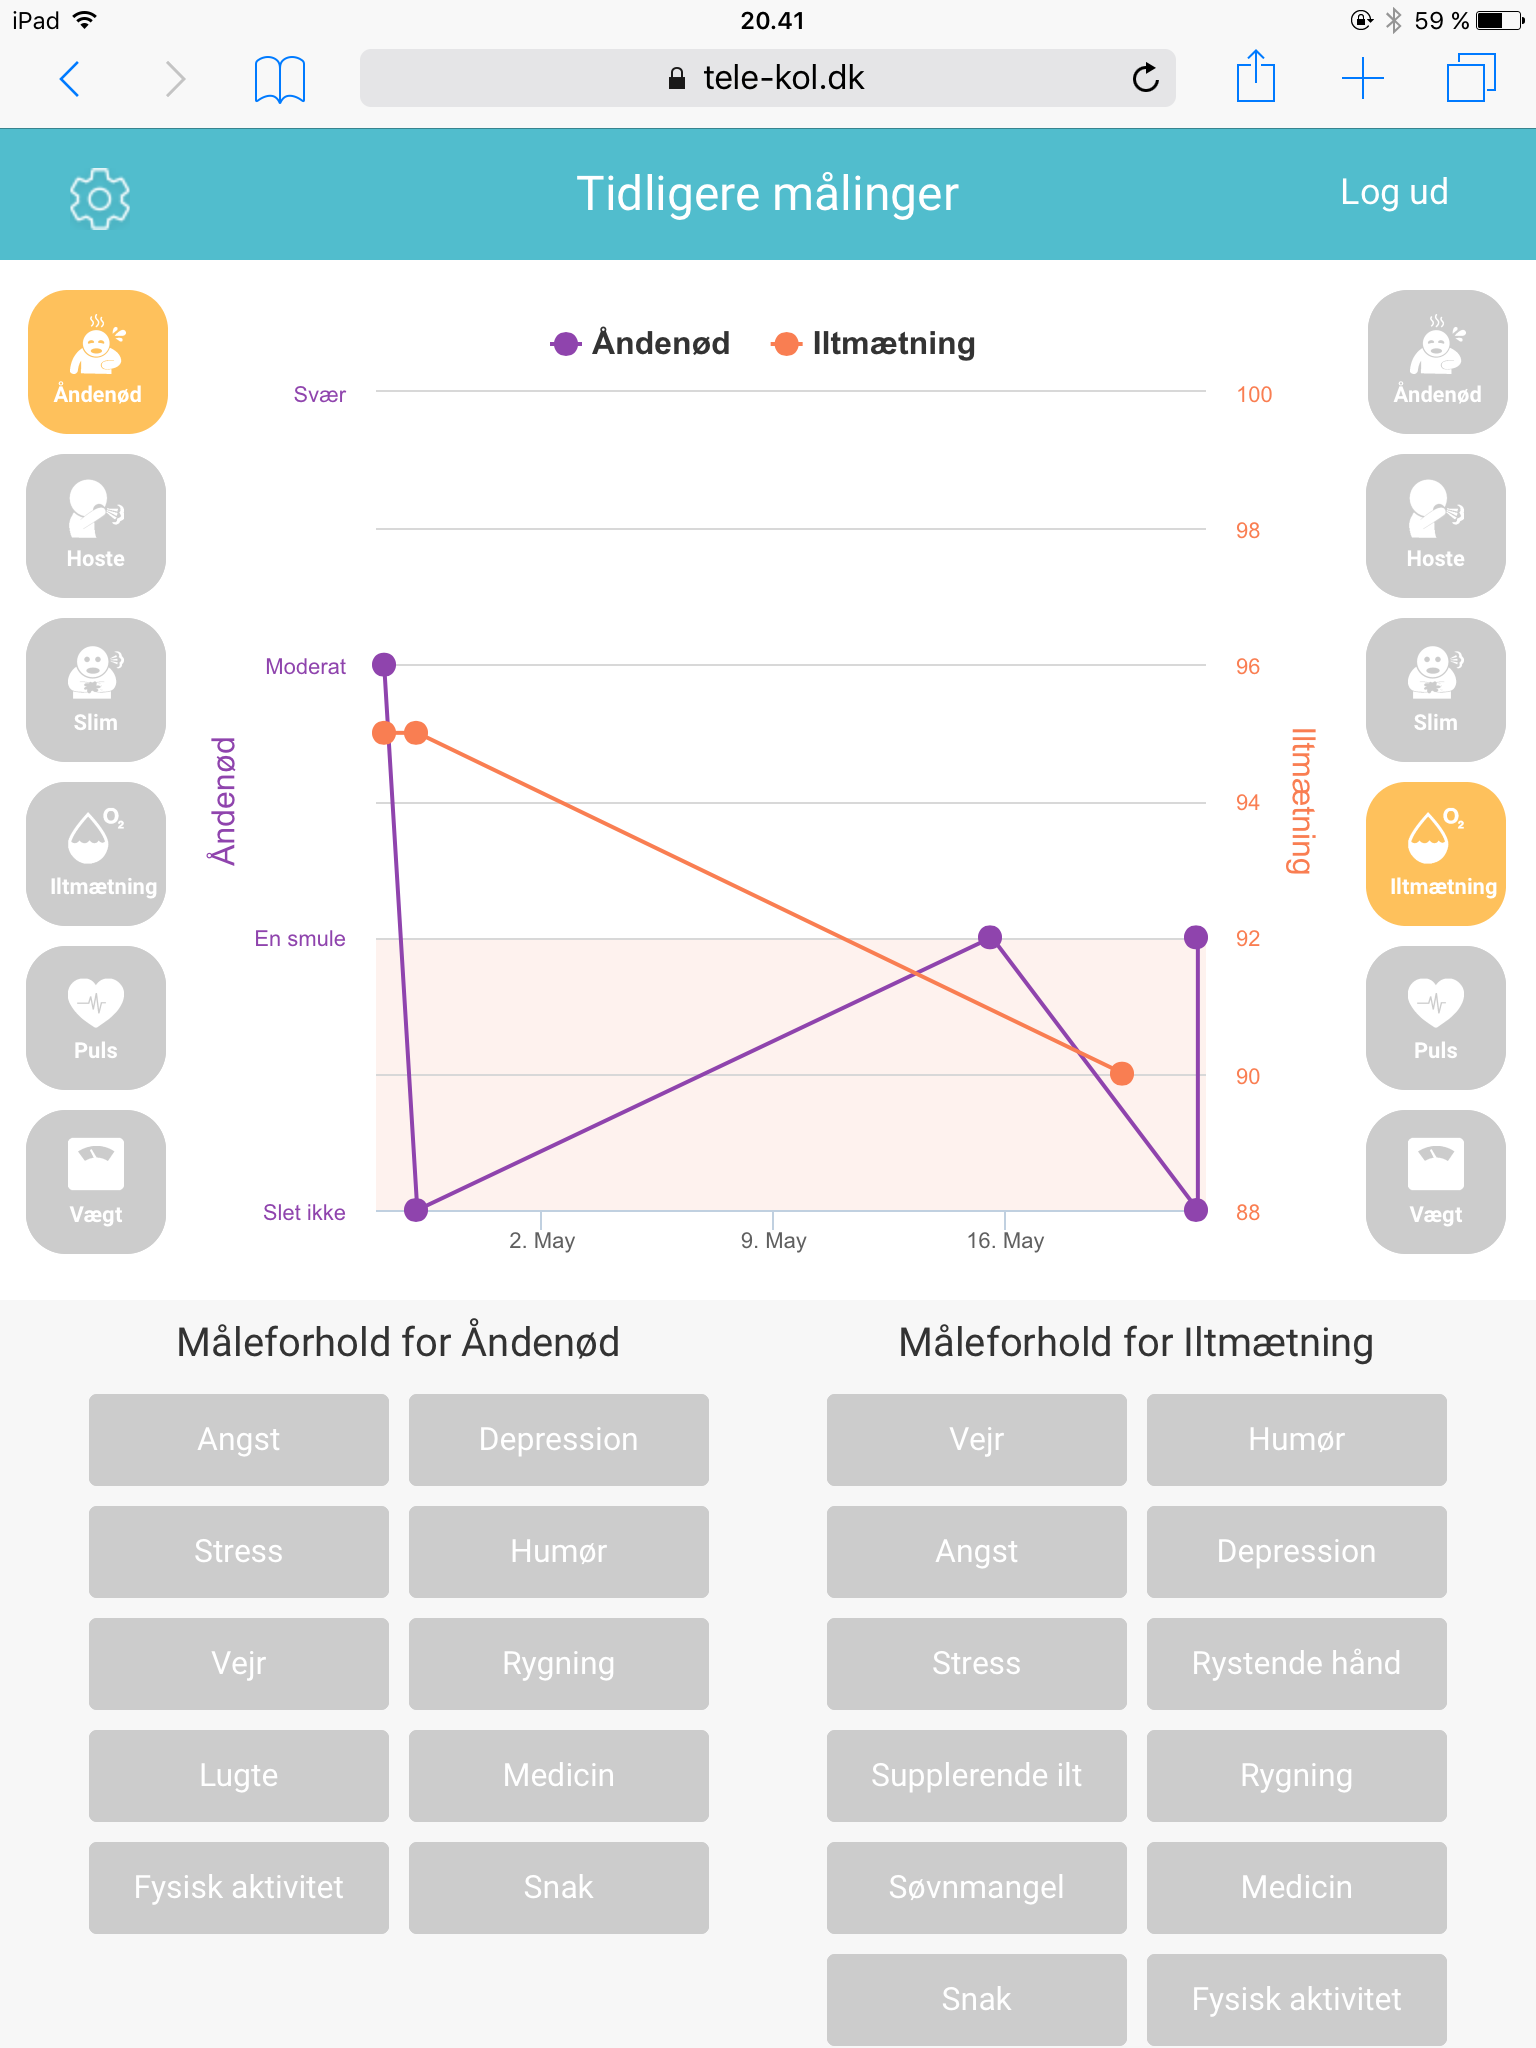
\includegraphics[width=\textwidth]{images/implementation/v1Imp.PNG}
    \caption{Visualisation 1}
    \label{fig:visualization}
  \end{minipage}
\end{figure}



\section{Server-side}


\subsection{Session}



\textbf{Admin Access}

admin features


\subsection{Data Manipulation}
data structure (json, log)
webservice - saveLatestQuestion

 
 
 
\section{Client-side}

\textbf{Get user data}

In order to get each user's data on login, we use ajax from the jquery library. 


\textbf{User Interface Elements}

The interface was built on the Bootstrap front-end framework \citep{bootstrap}. Bootstrap is open-source and provides HTML and CSS templates along with JavaScript components to design and build responsive web applications. For dashboard gauges we made use of the JavaScript plugin \textit{JustGage} \citep{justgage}, while we used \textit{Highcharts JS} \citep{highcharts} for visualising history data. 

Figure xxx shows an example of creating the gauge for cough with parameters customized for each measure (number of options for value, colors depending on current value, min and max text labels) 

Line 312 to 315 in app/index.php 

 
\section{Security}
anonymous
https
.htaccess
 - flaws
 - sufficient for trial, .. in operation use of database, programming convenience based on previous experience